\section{Hawker Sea Fury}

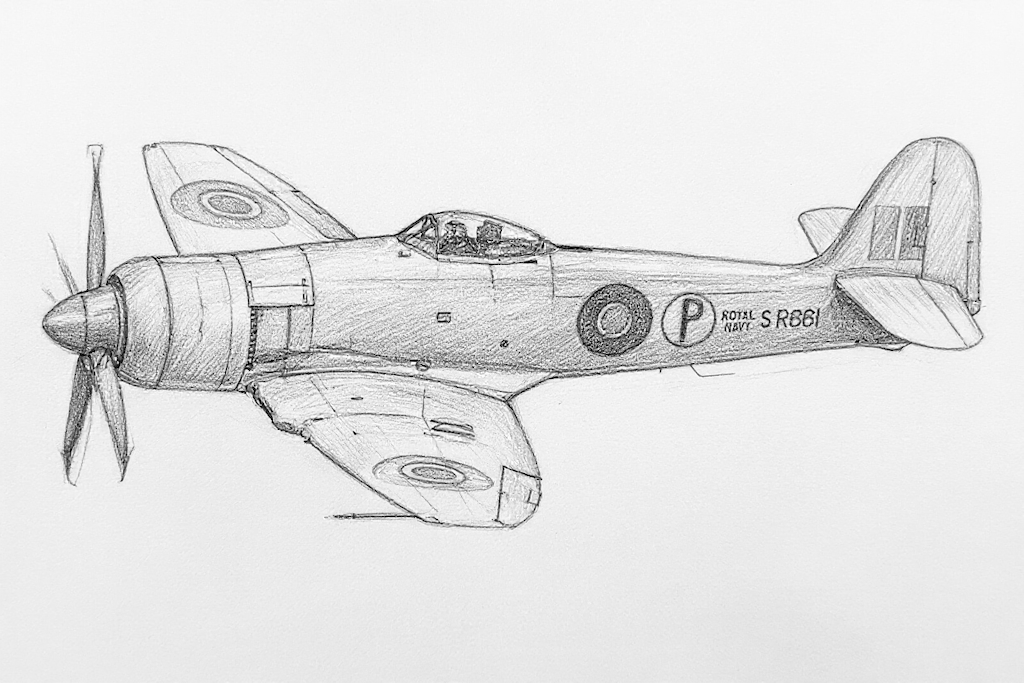
\includegraphics[width=\linewidth]{Sea Fury.png}

The Hawker Sea Fury is a post-WW2 propeller-driven fighter bomber.

The Sea Fury is a descendant of the WW2 Hawker Tempest fighter bomber, originally adapted as a long-range fighter for use in the war against Japan. After WW2 ended, the RAF no longer had interest, but the RN acquired a version adapted for carrier operations as a replacement for its Seafires, which were not well suited to carrier operations, and Corsairs, which had to be returned to the US as the Lend-Lease program ended. At the time, the high landing speeds of the first generation of jet aircraft was an impediment to their use on carriers. The Sea Fury is powered by a Centaur radial engine, armed with four 20 mm guns, and has a bubble canopy with an excellent view except under the nose.

\subsection{Versions}

\subsubsection{Sea Fury F.10}

The initial version of the Sea Fury is the F.10 day fighter.

It entered service in the RN in 1947, but seems to have been quickly replaced by the FB.11 version. It also served in the RAN and RCAF, although again might well have been quickly replaced by the FB.11.

\subsubsection{Sea Fury F.11}

The FB.11 is derived from the F.10 and has added armor and weapon stations to perform better as a fighter-bomber.

It served in the RN from 1948 to 1956, RAN from 1948 to 1959, and RCN from 1948 to 1956. Ex-RN aircraft served in the Cuban Air Force

\subsubsection{Sea Fury T.20}

The final version is the two-seater T.20 trainer.

RN, Iraq

\subsubsection{Sea Fury F.50, FB.50, and FB.51}

There are three major versions of the Sea Fury. The Sea Fury F.50, FB.50, and FB.51 and the Fury FB.60 are export versions of the F.10 and FB.11 with minor changes and removal of carrier-specific equipment from the FB.60.

The Sea Fury was exported to Australia, Burma, Canada, Cuba, Iraq, the Netherlands, and Pakistan. The RN and RAN used it as a fighter-bomber in the Korean War and also saw combat with the Cuban Revolutionary Air Force during the Bay of Pigs invasion and with the Netherlands Royal Navy in the Dutch East Indies. It was replaced in the RN by the Sea Hawk and Attacker starting in 1953, in the RCN by the F2H Banshees starting in 1956, and in the Netherlands Royal Navy by Sea Hawks.

A typical air-to-ground load is two 500-lb or 1000-lb bombs or twelve RP-3 rockets. It can also carry two 90-gallon fuel tanks to extend its range.

\subsection{ADC}

\begin{adclist}
    \adcitem{Sea Fury FB.11}
\end{adclist}

\subsection{Photo Credit}
\begin{itemize}\raggedright
    \item \href{https://commons.wikimedia.org/wiki/File:Hawker_Fury_FB.11_‘SR661’_(G-CBEL)_(35902999510).jpg}{Hawker Sea Fury}: Alan Wilson (CC BY-SA 2.0)
\end{itemize}
